\subsection{Paolo Penazzi}
Il mio compito all’interno del progetto è stato quello di modellare la gerarchia di Entity e Troop,
implementare le piante e l'attore che ne definisce il comportamento, realizzare i proiettili relativi alle piante e di generare le wave insieme a Parrinello.

\subsubsection{Troop}
Durante la modellazione delle Entity, insieme agli altri membri del gruppo è stato notato che il comportamento in comune tra le piante e gli zombie poteva essere definito in un concetto di Troop.

Grazie ai \textbf{mixin} mi è stato possibile definire il \texttt{trait Troop} come estensione del \texttt{trait Entity}
a cui viene aggiunta l'abilità di attaccare \texttt{AttackingAbility}.
Questo nuovo concetto di \texttt{Troop} ci ha permesso, in tutto il progetto, di trattare le piante e gli zombie allo stesso modo.

Durante l'analisi del dominio ho notato che le entità subiscono spesso modifiche durante la partita: l'aggiornamento della posizione, quello della vita o quello dello stato.
Ho quindi cercato un modo per rendere naturale questa modifica, che rispettasse però due vincoli:
\begin{itemize}
    \item Le entità devono essere immutabili.
    \item L'aggiornamento deve essere fatto in maniera funzionale.
\end{itemize}
Dopo vari tentativi con approcci differenti, la scelta è ricaduta sulla definizione di un metodo per ogni caratteristica da modificare: tale metodo prenderà in input il nuovo valore e restituirà una nuova troop con il campo aggiornato.

Questi metodi sono stati implementati utilizzando il metodo \textbf{copy} di Scala, che permette di fare proprio ciò di cui avevo bisogno.
L'unico difetto di questa soluzione è che il metodo \textit{copy} è disponibile sono nelle \textbf{case class}, quindi tutte le classi che estendono \textit{Troop} dovranno implementare quei metodi.

A questo punto la modifica di una troop può essere effettuata utilizzando la \textbf{notazione infissa}:

\begin{lstlisting}[language=Scala, label=code:troop-update, caption= Aggiornamento di una troop.]
    val troop: Troop
    val updatedTroop = troop withLife 50 withPosition (0,0)
\end{lstlisting}

Questa soluzione è stata poi adottata anche nei Bullet.

Gli stessi principi mi hanno guidato nella creazione di un modo di creare le troop che fosse il più funzionale possibile.
Ho quindi rivisitato il \textbf{pattern builder} per creare troop di qualsiasi tipo: ho creato un \texttt{trait TroopBuilder}
con un unico metodo \textit{build} che ritorna la troop desiderata.
Utilizzando le \textbf{given conversion} ho definito, per ogni possibile tipo di Troop, un'istanza del builder che si occupa
della creazione di quest'ultima.
Per rendere il builder più coerente con il linguaggio del progetto ho definito un metodo \textit{ofType} che che dato un tipo
di troop utilizza il builder per restituire la nuova entità.

\begin{lstlisting}[language=Scala, label=code:troop-builder, caption= Builder per la creazione di una Troop.]
    object Troops:
        trait TroopBuilder[T <: Troop, B <: Bullet]:
            def build: T

        given TroopBuilder[BasicZombie, Bullet] with
            override def build: BasicZombie = BasicZombie()

        given TroopBuilder[Wallnut, Bullet] with
            override def build: Wallnut = Wallnut()

        def ofType[T <: Troop](using troopBuilder: TroopBuilder[T, Bullet]): T =
            troopBuilder.build
\end{lstlisting}

Tutto ciò rende più funzionale la creazione di una troop, che può essere effettuata in questo modo:

\begin{lstlisting}[language=Scala, label=troop-creation, caption=Troop creation. ]
    val troop: Troop = Troops.ofType[BasicZombie]
\end{lstlisting}

L'idea di avere un builder per creare le entità del model è piaciuta al team, per questo ho implementato un secondo builder per creare \textit{Bullet}.
Non entrerò nel dettaglio in quanto per implementarlo, ho seguito il modello del \textit{TroopBuilder}.

\subsubsection{TroopActor}
Avendo adottato un'architettura ad attori, ogni troop, in fase di creazione, viene associata ad un attore che ne definisce il comportamento.
Il TroopActor ha un solo Behaviour e non è mai proattivo: risponde solamente ai messaggi ricevuti dal GameLoop, rispettando il pattern \textbf{MVC}.

Il punto di forza di questo \textit{Troop Actor} è che modella il comportamento delle piante e degli zombie come se fossero equivalenti.
Questo conferma le scelte di design fatte, in particolare quella di creare un \textit{trait troop} comune sia alle piante che agli zombie.

Ad ogni iterazione del GameLoop il TroopActor riceve un messaggio di \textit{Update()} a seguito del quale:
\begin{itemize}
    \item Aggiorna la propria troop.
    \item Se la troop ha raggiunto la fine della corsia notifica il GameLoop.
    \item Manda la troop aggiornata al GameLoop.
    \item Se c'è un nemico attaccabile, manda a se stesso un messaggio Shoot().
    \item Ricrea il proprio Behaviour con la troop aggiornata.
\end{itemiza}

Nel caso ci sia un'entità da attaccare, riceverà il messaggio Shoot(), che si è precedentemente inviato, a seguito del quale:

\begin{itemize}
    \item Crea il bullet che la propria troop spara.
    \item Crea un BulletActor che controlla il bullet.
    \item Notifica il GameLoop dell'avvenuta creazione inviandogli il messaggio BulletSpawned(), contenente il riferimento al bullet e al BulletActor.
\end{itemize}

Nel caso la troop venga colpita da un bullet, il TroopActor viene notificato dal GameLoop con il messaggio Collision(), a seguito del quale:

\begin{itemize}
    \item Applica il danno e l'eventuale effetto del bullet alla troop.
    \item Se la troop viene uccisa, risponde con il messaggio EntityDead()
    \item Se la troop non viene uccisa, risponde con il messaggio EntityUpdated()
\end{itemize}

Il comportamento del TroopActor viene mostrato nel seguente diagramma:

\begin{figure}[H]
    \centering
    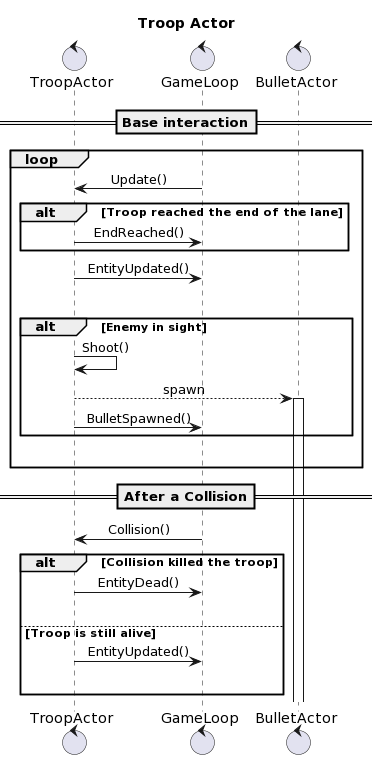
\includegraphics[width=0.8\linewidth]{images/troop-actor.png}
    \label{Diagramma di sequenza del Troop Actor.}
\end{figure}

\subsubsection{Plant}
Un'altra parte fondamentale del mio lavoro è stata la creazione dei vari tipi di piante: sono partito definendo un \texttt{trait Plant} che estende \textit{Troop} e modella il comportamento comune tra le varie piante.
Ho poi creato vari tipi di piante creando delle classi che estendono \textit{Plant}.

Durante l'implementazione di queste classi, ho notato che tutte le piante che sparano hanno lo stesso comportamente, l'unica cosa che cambia è il bullet che sparano.
Ogni tipo di pianta che spara può essere quindi identificata dal rispettivo bullet.

Ho cercato di migliorare la mia implementazione, provando a renderla il più riusabile possibile per non ripetere codice: ho tentato vari approcci, dall'utilizzo di classi astratte alla delegazione, ognuno dei quali presentava vantaggi e svantaggi.
La scelta finale è ricaduta sull'utilizzo di una \textbf{type class} che modella le piante che sparano.

Ho creato la classe \textit{Shooter} che è una type class generica sul tipo di bullet che spara.
Questa implementazione è stata possibile grazie all'utilizzo, nel \textit{trait Plant}, di un \textbf{abstract type} \textit{BulletType \textless: Bullet} per definire il tipo di ritorno del metodo \textit{bullet}.

\begin{lstlisting}[language=Scala, label=code:plant-shooter caption=Type class Shooter.]
case class Shooter[B <: Bullet]
    (bulletInstance: B,
    override val position: Position = (0, 0),
    override val life: Int = shooterDefaultLife,
    override val state: TroopState = defaultPlantState)
    extends Plant :

  override type BulletType = B
\end{lstlisting}

Per istanziare questa pianta ho definito un metodo ad-hoc, che sotto utilizza il \textit{TroopBuilder} definito in precedenza.
È quindi possibile creare shooter nella seguente maniera:

\begin{lstlisting}[language=Scala, label=shooter-builder, caption=Shooter creation. ]
    val plant: Plant = Troops.shooterOf[PeaBullet]
\end{lstlisting}

In questa classe non rientrano due tipi di piante, il \texttt{wallnut} e la \texttt{cherry bomb}.
Queste sono state implementate utilizzando classi ad-hoc perchè hanno un comportamente diverso rispetto alle piante che sparano:
\begin{itemize}
    \item Il Wallnut è una pianta con tanta vita che però non può attaccare.
    \item La Cherrybomb è una pianta che quando piazzata esplode, colpendo tutti i tipi di \textit{Troop}.
\end{itemize}

Tutti i valori relativi alle piante (defaultLife, bullet, etc..) sono stati inseriti in un oggetto \texttt{PlantDefaultValues},
in modo da rendere più pulito il codice e facilitare il bilanciamento del gioco.

\begin{lstlisting}[language=Scala, label=default-values, caption=Plant default values.]
      val shooterDefaultLife: Int = 100
      val wallnutDefaultLife: Int = 150

      val bullets: Plant => PlantBullet =
        case s: Shooter[_] =>
        s.bulletInstance match
          case _: PeaBullet => Bullets.ofType[PeaBullet]
          case _: SnowBullet => Bullets.ofType[SnowBullet]
        case c: CherryBomb => CherryBullet(c.position)
\end{lstlisting}

Il diagramma della gerarchia delle piante è il seguente:

\begin{figure}[H]
    \centering
    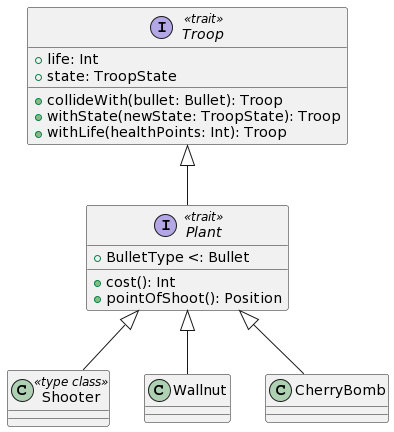
\includegraphics[width=0.8\linewidth]{images/plants.png}
    \label{Diagramma delle classi delle piante.}
\end{figure}

A seguito del mio lavoro sulle piante ho anche implementato i bullet relativi e contribuito, in maniera significativa, alla modellazione di questi ultimi.
